%%%%%%%%%%%%%%%%%%%%%%%%%%%%%%%%%%%%%%%%%%%%%%%%%%%%%%%%%%%%%%%%%%%%%%%%%%%%%%%%%%%%%%%%%%%%%%%%%%%
%%%%%%%%%%%%%%%%%%%%%%%%%%%%%%%%%%%%%%%%%%%%%%%%%%%%%%%%%%%%%%%%%%%%%%%%%%%%%%%%%%%%%%%%%%%%%%%%%%%
\chapter{Resultados}

%Como se mencion\'o previamente, este trabajo se ha basado en los registros de PSG de 6 adultos
%mayores con deterioro cognitivo (DC) y 3 sin este padecimiento. La calidad de deterioro
%cognitivo fue medida a trav\'es de una bater\'ia de pruebas neuropsicol\'ogicas;
%adicionalmente, se midi\'o su posible depresi\'on geri\'atrica. 
%En e cuadro \ref{sujetos} se resume esta informaci\'on.
%
%\begin{table}
%\centering
%\begin{tabular}{l|cc}
%Sujeto & Deterioro cogn. & Depresi\'on
%\\
%\hline
%MJNN &   &   \\
%RLMN & X &   \\
%JANA &   & X \\
%CLMN & X &   \\
%JGMN & X &   \\
%RRMN & X &   \\
%VCNN &   &   \\
%FGH  & X & ? \\
%GURM & ? & ? \\
%%& & \\
%%& & \\
%\end{tabular}
%\caption{Caracter\'isticas de los adultos mayores considerados en el estudio, en cuanto
%a deterioro cognitivo y depresi\'on geri\'atrica. 
%%Las dos primeras letras fueron dadas por sus nombre mientras que las \'ultimas dos son
%%mnemotecnias de sus caracter\'isticas: \textbf{M}= mean, \textbf{N}=normal, \textbf{A}=anormal.
%Para m\'as detalles consultar \cite{VazquezTagle16}}
%\label{sujetos}
%\end{table}

%Estos gr\'aficos muestran una distribuci\'ion temporal y pseudo-espacial 
%de las \'epocas que fueron clasificadas como {no-estacionarias} seg\'un el test PSR
%(ver seccipara m\'as detalles). 
%%M\'as que eso, esta distribuci\'on gr\'afica puede extenderse a otros an\'alisis.

En cada canal que conforma el PSG (EEG, EOG y EMG), 
cada una de las \'epocas consideradas fue clasificada como 
''\'Epoca Posiblemente Estacionaria'' (EPE) si no pudo ser rechazado la hip\'otesis de 
estacionariedad usando el test PSR ($\alpha = 0.05$), mientra que 
%el rechazo de esta misma 
%hip\'otesis es argumento ''suficiente'' para afirmar que el segmento de registro en cuenti\'on
%puede ser clasificado omo no.estacionario.
fue clasificado como ''No-estacionario'' en caso contrario. Variar el valor cr\'itico
para la clasificaci\'on no parece generar diferencias significativas.



Una debilidad importante de los gr\'aficos as\'i obtenidos es que, si bien muestran patrones 
claros en el tiempo, \'estos no se pueden cuantificar de una manera obvia y se dificulta la
comparaci\'on entre sujetos. Se han inclu\'ido estos resultados porque sus caracter\'isticas 
sugieren una posible utilizaci\'on para otros fines --en alg\'un trabajo futuro.

La cantidad de \'epocas que no fueron para las cuales no es posible rechazar la hip\'otesis de
estacionariedad ($\alpha=0.05$)
clasificadas como ''\'Epocas Posiblemente Estacionarias'' (EPE).
Como un segundo an\'alisis,
la proporci\'on de EPE con respecto al total de \'epocas registradas fue comparado contra la misma
cantidad restringida \'unicamente a \'epocas correspondientes a sue\~no MOR; la comparaci\'on 
se realiz\'o usando una prueba $\chi^{2}$ de proporciones.
%Tanto las proporciones como las diferencias significativas se encuentran en la tabla

%\begin{table}
%\centering
%\begin{tabularx}{\hsize}{c|cc|cc|cc}
%Canal&Total&&NMOR&&MOR&\\
%&Estacionarios&Porcentaje&Estacionarios&Porcentaje&Estacionarios&Porcentaje\\
%\hline
%C3&325&31.6\%&285&33.0\%&40&24.1\%\\
%C4&339&32.9\%&306&35.4\%&33&19.9\%\\
%CZ&318&30.9\%&289&33.4\%&29&17.5\%\\
%EMG&96&9.3\%&91&10.5\%&5&3.0\%\\
%F3&247&24.0\%&220&25.5\%&27&16.3\%\\
%F4&241&23.4\%&233&27.0\%&8&4.8\%\\
%F7&220&21.4\%&214&24.8\%&6&3.6\%\\
%F8&196&19.0\%&194&22.5\%&2&1.2\%\\
%FP1&244&23.7\%&243&28.1\%&1&0.6\%\\
%FP2&234&22.7\%&232&26.9\%&2&1.2\%\\
%FZ&298&28.9\%&271&31.4\%&27&16.3\%\\
%LOG&556&54.0\%&541&62.6\%&15&9.0\%\\
%O1&271&26.3\%&239&27.7\%&32&19.3\%\\
%O2&279&27.1\%&255&29.5\%&24&14.5\%\\
%P3&349&33.9\%&313&36.2\%&36&21.7\%\\
%P4&327&31.7\%&301&34.8\%&26&15.7\%\\
%PZ&295&28.6\%&278&32.2\%&17&10.2\%\\
%ROG&581&56.4\%&553&64.0\%&28&16.9\%\\
%T3&221&21.5\%&174&20.1\%&47&28.3\%\\
%T4&206&20.0\%&193&22.3\%&13&7.8\%\\
%T5&362&35.1\%&304&35.2\%&58&34.9\%\\
%T6&323&31.4\%&301&34.8\%&22&13.3\%\\
%\end{tabularx}
%\end{table}


\begin{table}
\centering
\begin{tabular}{c|ccccc|cc}
& VCR & MJH & JAE & GHA? & MFGR? & $\widehat{\mu}$ & $\widehat{\sigma}$ \\
\hline
 C3 & 0.082    & 0.142    & 0.047    & 0.189    && 0.115    & 0.063     \\
 C4 & 0.096    & 0.126    & 0.006    & 0.126    && 0.089    & 0.057     \\
 CZ & 0.027    & 0.126    & 0.006    & 0.095    && 0.063    & 0.056     \\
 F3 & 0.068    & 0.181    & 0.018    & 0.147    && 0.104    & 0.074     \\
 F4 & 0.151    & 0.181    & -      & 0.168    && 0.125    & 0.084     \\
 F7 & 0.068    & 0.118    & 0.006    & 0.232    && 0.106    & 0.095     \\
 F8 & 0.055    & 0.087    & -      & 0.242    && 0.096    & 0.104     \\
 FP1 & 0.027    & 0.055    & 0.058    & 0.253    && 0.098    & 0.104     \\ 
 FP2 & 0.014    & 0.047    & 0.006    & 0.105    && 0.043    & 0.045     \\ 
 FZ & 0.151    & 0.142    & 0.012    & 0.126    && 0.108    & 0.065     \\
 O1 & 0.137    & 0.157    & -      & 0.284    && 0.145    & 0.116     \\
 O2 & 0.178    & 0.181    & -      & 0.274    && 0.158    & 0.114     \\
 P3 & 0.082    & 0.134    & -      & 0.263    && 0.120    & 0.110     \\
 P4 & 0.055    & 0.150    & -      & 0.295    && 0.125    & 0.129     \\
 PZ & 0.055    & 0.118    & -      & 0.221    && 0.098    & 0.095     \\
 T3 & 0.137    & 0.228    & -      & 0.274    && 0.160    & 0.121     \\
 T4 & 0.164    & 0.157    & -      & 0.116    && 0.109    & 0.076     \\
 T5 & 0.137    & 0.205    & -      & 0.211    && 0.138    & 0.098     \\
 T6 & 0.205    & 0.142    & -      & 0.263    && 0.153    & 0.113     \\
 LOG & 0.082    & 0.157    & 0.018    & 0.263    && 0.130    & 0.106     \\
 ROG & 0.082    & 0.165    & 0.006    & 0.316    && 0.142    & 0.133     \\
 EMG & 0.192    & 0.087    & 0.012    & -      && 0.073    & 0.088    
\end{tabular}
\caption{Proporci\'on estimada de \'epocas PE respecto al total de \'epocas MOR 
(fase R) en cada
canal, para el grupo \textit{Normal}.}
\label{gpo_NN_mor}
\end{table}

\begin{table}
\centering
\begin{tabular}{c|cccc|cc}
& CLO & RLO & RRU & JGZ & $\widehat{\mu}$ & $\widehat{\sigma}$ \\
\hline
 C3 &0.045    &0.354    &0.421    &0.030    &0.213    &0.204     \\
 C4 &0.030    &0.404    &0.132    &-    &0.141    &0.184     \\
 CZ &0.038    &0.222    &0.105    &0.030    &0.099    &0.089    \\ 
 F3 &0.053    &0.434    &0.079    &0.091    &0.164    &0.181     \\
 F4 &0.045    &0.364    &0.132    &-    &0.135    &0.162     \\
 F7 &0.008    &0.182    &-    &-    &0.047    &0.090     \\
 F8 &0.030    &0.232    &0.026    &-    &0.072    &0.108    \\ 
 FP1 &-    &-    &0.026    &-    &0.007    &0.013     \\
 FP2 &0.008    &0.152    &0.026    &-    &0.046    &0.071     \\
 FZ &0.053    &0.384    &0.053    &0.061    &0.138    &0.164     \\
 O1 &0.015    &0.253    &0.237    &0.061    &0.141    &0.121     \\
 O2 &0.023    &0.343    &0.237    &0.030    &0.158    &0.158     \\
 P3 &0.038    &0.333    &0.211    &-    &0.145    &0.155     \\
 P4 &0.030    &0.273    &0.132    &0.030    &0.116    &0.115    \\ 
 PZ &0.030    &0.323    &0.105    &-    &0.115    &0.146     \\
 T3 &0.076    &0.343    &0.105    &-    &0.131    &0.148     \\
 T4 &0.023    &0.354    &0.158    &0.030    &0.141    &0.155     \\
 T5 &0.038    &0.343    &0.132    &0.061    &0.143    &0.139     \\
 T6 &0.023    &0.242    &0.105    &0.061    &0.108    &0.096     \\
 LOG &0.038    &0.111    &0.053    &-    &0.050    &0.046     \\
 ROG &0.068    &0.071    &0.105    &0.030    &0.069    &0.031    \\ 
 EMG &0.106    &0.162    &0.105    &-    &0.093    &0.068    
\end{tabular}
\caption{Proporci\'on estimada de \'epocas PE respecto al total de \'epocas
MOR (fase R) en cada
canal, para el grupo \textit{PDC}.}
\label{gpo_mn_mor}
\end{table}

\begin{table}
\centering
\begin{tabular}{c|ccc}
& FGH & MGG & EMT \\
 C3 & 0.091    & 0.169    & 0.191     \\
 C4 & 0.045    & 0.139    & 0.213     \\
 CZ & 0.045    & 0.078    & 0.255     \\
 F3 & 0.273    & 0.084    & 0.085     \\
 F4 & -      & 0.024    & 0.319     \\
 F7 & -      & 0.012    & 0.043     \\
 F8 & -      & 0.012    & 0.234     \\
 FP1 & 1.000    & -      & 0.170     \\
 FP2 & -      & 0.006    & 0.085     \\
 FZ & -      & 0.120    & 0.298     \\
 O1 & 0.227    & 0.108    & 0.277     \\
 O2 & 0.045    & 0.072    & 0.106     \\
 P3 & 0.045    & 0.145    & 0.234     \\
 P4 & 0.182    & 0.090    & 0.234     \\
 PZ & 0.045    & 0.048    & 0.149     \\
 T3 & 0.091    & 0.175    & 0.149     \\
 T4 & -      & 0.060    & 0.277     \\
 T5 & 0.091    & 0.187    & 0.319     \\
 T6 & -      & 0.054    & 0.234     \\
 LOG & 0.045    & 0.048    & 0.277     \\
 ROG & -      & 0.114    & 0.340     \\
 EMG & -      & 0.018    & 0.021    
\end{tabular}
\caption{Proporci\'on estimada de \'epocas PE respecto al total de \'epocas
MOR (fase R) en cada
canal, para los sujetos \textit{excluidos}.}
\label{gpo_zz_mor}
\end{table}

\begin{table}
\centering
\begin{tabular}{c|ccccc|cc}
& VCR & MJH & JAE & GHA? & MFGR? & $\widehat{\mu}$ & $\widehat{\sigma}$ \\
\hline
 C3 & 0.237    & 0.149    & 0.030    & 0.160    && 0.144    & 0.086    \\ 
 C4 & 0.213    & 0.143    & 0.033    & 0.146    && 0.134    & 0.075     \\
 CZ & 0.212    & 0.145    & 0.030    & 0.100    && 0.122    & 0.077     \\
 F3 & 0.213    & 0.148    & 0.037    & 0.136    && 0.134    & 0.073     \\
 F4 & 0.228    & 0.146    & 0.024    & 0.131    && 0.133    & 0.084     \\
 F7 & 0.201    & 0.151    & 0.039    & 0.191    && 0.146    & 0.074     \\
 F8 & 0.199    & 0.136    & 0.019    & 0.146    && 0.125    & 0.076     \\
 FP1 & 0.207    & 0.083    & 0.018    & 0.100    && 0.102    & 0.078     \\
 FP2 & 0.198    & 0.091    & 0.027    & 0.106    && 0.105    & 0.070     \\
 FZ & 0.216    & 0.148    & 0.034    & 0.144    && 0.136    & 0.075     \\
 O1 & 0.256    & 0.192    & 0.023    & 0.272    && 0.186    & 0.114     \\
 O2 & 0.211    & 0.182    & 0.023    & 0.224    && 0.160    & 0.093     \\
 P3 & 0.222    & 0.135    & 0.012    & 0.266    && 0.159    & 0.112     \\
 P4 & 0.228    & 0.150    & 0.034    & 0.229    && 0.161    & 0.092     \\
 PZ & 0.198    & 0.145    & 0.019    & 0.199    && 0.140    & 0.085     \\
 T3 & 0.230    & 0.155    & 0.027    & 0.212    && 0.156    & 0.092     \\
 T4 & 0.230    & 0.134    & 0.015    & 0.180    && 0.140    & 0.092     \\
 T5 & 0.277    & 0.161    & -      & 0.248    && 0.172    & 0.124     \\
 T6 & 0.277    & 0.164    & 0.023    & 0.193    && 0.164    & 0.106     \\
 LOG & 0.299    & 0.248    & 0.118    & 0.263    && 0.232    & 0.079     \\
 ROG & 0.299    & 0.227    & 0.091    & 0.307    && 0.231    & 0.100     \\
 EMG & 0.119    & 0.069    & 0.005    & 0.002    && 0.049    & 0.056    
\end{tabular}
\caption{Proporci\'on estimada de \'epocas PE respecto al total de \'epocas no-MOR
(fases W y N) en cada
canal, para el grupo \textit{Normal}.}
\label{gpo_NN_nmor}
\end{table}

\begin{table}
\centering
\begin{tabular}{c|cccc|cc}
& CLO & RLO & RRU & JGZ & $\widehat{\mu}$ & $\widehat{\sigma}$ \\
\hline
 C3 & 0.068    & 0.205    & 0.202    & 0.048    & 0.131    & 0.085     \\
 C4 & 0.044    & 0.181    & 0.250    & 0.040    & 0.129    & 0.104     \\
 CZ & 0.067    & 0.194    & 0.184    & 0.053    & 0.124    & 0.075     \\
 F3 & 0.070    & 0.234    & 0.210    & 0.058    & 0.143    & 0.092     \\
 F4 & 0.050    & 0.181    & 0.213    & 0.042    & 0.121    & 0.088     \\
 F7 & 0.055    & 0.150    & 0.181    & 0.049    & 0.109    & 0.066     \\
 F8 & 0.050    & 0.129    & 0.229    & 0.041    & 0.112    & 0.087     \\
 FP1 & 0.042    & -      & 0.189    & 0.037    & 0.067    & 0.083     \\
 FP2 & 0.041    & 0.133    & 0.069    & 0.037    & 0.070    & 0.044     \\
 FZ & 0.068    & 0.218    & 0.242    & 0.055    & 0.146    & 0.098     \\
 O1 & 0.059    & 0.201    & 0.245    & 0.082    & 0.147    & 0.090     \\
 O2 & 0.039    & 0.182    & 0.186    & 0.090    & 0.124    & 0.072     \\
 P3 & 0.089    & 0.197    & 0.287    & 0.081    & 0.163    & 0.098     \\
 P4 & 0.069    & 0.181    & 0.293    & 0.062    & 0.151    & 0.109     \\
 PZ & 0.070    & 0.224    & 0.298    & 0.050    & 0.160    & 0.120     \\
 T3 & 0.100    & 0.150    & 0.213    & 0.087    & 0.137    & 0.057     \\
 T4 & 0.032    & 0.147    & 0.298    & 0.074    & 0.138    & 0.117     \\
 T5 & 0.096    & 0.183    & 0.277    & 0.052    & 0.152    & 0.099     \\
 T6 & 0.047    & 0.158    & 0.261    & 0.072    & 0.134    & 0.097     \\
 LOG & 0.177    & 0.248    & 0.340    & 0.192    & 0.239    & 0.074     \\
 ROG & 0.155    & 0.240    & 0.293    & 0.192    & 0.220    & 0.060     \\
 EMG & 0.025    & 0.110    & 0.293    & 0.009    & 0.109    & 0.130    
\end{tabular}
\caption{Proporci\'on estimada de \'epocas PE respecto al total de \'epocas
no-MOR (fases W y N) en cada
canal, para el grupo \textit{PDC}.}
\label{gpo_mn_nmor}
\end{table}

\begin{table}
\centering
\begin{tabular}{c|ccc}
& FGH & MGG & EMT \\
 C3 & 0.042    & 0.233    & 0.142     \\
 C4 & 0.018    & 0.240    & 0.181     \\
 CZ & 0.021    & 0.208    & 0.138     \\
 F3 & 0.279    & 0.166    & 0.091     \\
 F4 & -      & 0.159    & 0.179     \\
 F7 & -      & 0.176    & 0.079     \\
 F8 & -      & 0.148    & 0.181     \\
 FP1 & 0.995    & 0.196    & 0.142     \\
 FP2 & -      & 0.169    & 0.110     \\
 FZ & -      & 0.205    & 0.171     \\
 O1 & 0.052    & 0.162    & 0.242     \\
 O2 & 0.057    & 0.186    & 0.209     \\
 P3 & 0.076    & 0.245    & 0.130     \\
 P4 & 0.047    & 0.238    & 0.144     \\
 PZ & 0.039    & 0.205    & 0.128     \\
 T3 & 0.070    & 0.133    & 0.175     \\
 T4 & 0.026    & 0.141    & 0.138     \\
 T5 & 0.050    & 0.241    & 0.215     \\
 T6 & 0.047    & 0.242    & 0.234     \\
 LOG & 0.131    & 0.506    & 0.352     \\
 ROG & 0.175    & 0.527    & 0.413     \\
 EMG & 0.003    & 0.064    & 0.083   
\end{tabular}
\caption{Proporci\'on estimada de \'epocas PE respecto al total de \'epocas
no-MOR (fases W y R) en cada
canal, para los sujetos \textit{excluidos}.}
\label{gpo_zz_nmor}
\end{table}

\begin{table}
\centering
\begin{tabular}{c|ccccc|cc}
& VCR & MJH & JAE & GHA? & MFGR? & $\widehat{\mu}$ & $\widehat{\sigma}$ \\
\hline
 C3 & 0.224    & 0.148    & 0.033    & 0.163    && 0.142    & 0.080    \\
 C4 & 0.203    & 0.141    & 0.028    & 0.145    && 0.129    & 0.073    \\
 CZ & 0.196    & 0.142    & 0.025    & 0.100    && 0.116    & 0.072    \\
 F3 & 0.201    & 0.152    & 0.033    & 0.137    && 0.131    & 0.071    \\
 F4 & 0.222    & 0.150    & 0.020    & 0.134    && 0.132    & 0.084    \\
 F7 & 0.189    & 0.147    & 0.033    & 0.195    && 0.141    & 0.075    \\
 F8 & 0.187    & 0.130    & 0.015    & 0.155    && 0.122    & 0.075    \\
 FP1 & 0.192    & 0.079    & 0.025    & 0.113    && 0.102    & 0.070    \\
 FP2 & 0.182    & 0.085    & 0.023    & 0.106    && 0.099    & 0.066    \\
 FZ & 0.210    & 0.147    & 0.030    & 0.143    && 0.133    & 0.075    \\
 O1 & 0.246    & 0.188    & 0.019    & 0.273    && 0.181    & 0.114    \\
 O2 & 0.208    & 0.182    & 0.019    & 0.229    && 0.159    & 0.096    \\
 P3 & 0.210    & 0.135    & 0.010    & 0.265    && 0.155    & 0.111    \\
 P4 & 0.214    & 0.150    & 0.028    & 0.235    && 0.157    & 0.093    \\
 PZ & 0.186    & 0.141    & 0.015    & 0.201    && 0.136    & 0.084    \\
 T3 & 0.222    & 0.164    & 0.022    & 0.218    && 0.156    & 0.093    \\
 T4 & 0.224    & 0.137    & 0.012    & 0.175    && 0.137    & 0.091    \\
 T5 & 0.265    & 0.167    & -      & 0.245    && 0.169    & 0.120    \\
 T6 & 0.271    & 0.161    & 0.019    & 0.199    && 0.162    & 0.106    \\
 LOG & 0.281    & 0.236    & 0.099    & 0.263    && 0.220    & 0.082    \\
 ROG & 0.281    & 0.219    & 0.075    & 0.307    && 0.221    & 0.104    \\
 EMG & 0.125    & 0.071    & 0.007    & 0.002    && 0.051    & 0.059
\end{tabular}
\caption{Proporci\'on estimada de \'epocas PE respecto al total de \'epocas
registradas (todas las fases) en cada
canal, para el grupo \textit{Normal}.}
\label{gpo_NN_tot}
\end{table}

\begin{table}
\centering
\begin{tabular}{c|cccc|cc}
& CLO & RLO & RRU & JGZ & $\widehat{\mu}$ & $\widehat{\sigma}$ \\
\hline
 C3 & 0.065    & 0.222    & 0.222    & 0.047    & 0.139    & 0.096     \\
 C4 & 0.042    & 0.207    & 0.239    & 0.039    & 0.132    & 0.106     \\
 CZ & 0.063    & 0.197    & 0.176    & 0.052    & 0.122    & 0.075     \\
 F3 & 0.068    & 0.258    & 0.198    & 0.059    & 0.146    & 0.098     \\
 F4 & 0.050    & 0.202    & 0.205    & 0.041    & 0.124    & 0.092     \\
 F7 & 0.049    & 0.154    & 0.164    & 0.048    & 0.104    & 0.064     \\
 F8 & 0.048    & 0.141    & 0.210    & 0.040    & 0.110    & 0.081     \\
 FP1 & 0.036    & -      & 0.174    & 0.036    & 0.062    & 0.077     \\
 FP2 & 0.036    & 0.135    & 0.065    & 0.036    & 0.068    & 0.046     \\
 FZ & 0.066    & 0.238    & 0.225    & 0.056    & 0.146    & 0.099     \\
 O1 & 0.053    & 0.207    & 0.244    & 0.081    & 0.146    & 0.093     \\
 O2 & 0.037    & 0.201    & 0.191    & 0.089    & 0.129    & 0.080     \\
 P3 & 0.082    & 0.213    & 0.280    & 0.079    & 0.163    & 0.100     \\
 P4 & 0.064    & 0.191    & 0.278    & 0.061    & 0.149    & 0.105     \\
 PZ & 0.065    & 0.235    & 0.280    & 0.049    & 0.157    & 0.118     \\
 T3 & 0.096    & 0.173    & 0.203    & 0.085    & 0.139    & 0.058     \\
 T4 & 0.031    & 0.171    & 0.285    & 0.073    & 0.140    & 0.113     \\
 T5 & 0.088    & 0.202    & 0.263    & 0.052    & 0.151    & 0.098     \\
 T6 & 0.043    & 0.168    & 0.246    & 0.071    & 0.132    & 0.093     \\
 LOG & 0.158    & 0.232    & 0.314    & 0.186    & 0.222    & 0.068     \\
 ROG & 0.143    & 0.220    & 0.275    & 0.187    & 0.206    & 0.056     \\
 EMG & 0.036    & 0.116    & 0.275    & 0.008    & 0.109    & 0.120   
\end{tabular}
\caption{Proporci\'on estimada de \'epocas PE respecto al total de \'epocas
registradas (todas las fases) en cada
canal, para el grupo \textit{PDC}.}
\label{gpo_mn_tot}
\end{table}

\begin{table}
\centering
\begin{tabular}{c|ccc}
& FGH & MGG & EMT \\
 C3 & 0.044    & 0.222    & 0.146     \\
 C4 & 0.020    & 0.223    & 0.184     \\
 CZ & 0.022    & 0.187    & 0.148     \\
 F3 & 0.279    & 0.152    & 0.090     \\
 F4 & -      & 0.137    & 0.191     \\
 F7 & -      & 0.150    & 0.076     \\
 F8 & -      & 0.126    & 0.186     \\
 FP1 & 0.995    & 0.164    & 0.144     \\
 FP2 & -      & 0.143    & 0.108     \\
 FZ & -      & 0.191    & 0.182     \\
 O1 & 0.062    & 0.153    & 0.245     \\
 O2 & 0.057    & 0.168    & 0.200     \\
 P3 & 0.074    & 0.229    & 0.139     \\
 P4 & 0.054    & 0.215    & 0.151     \\
 PZ & 0.040    & 0.180    & 0.130     \\
 T3 & 0.072    & 0.140    & 0.173     \\
 T4 & 0.025    & 0.128    & 0.150     \\
 T5 & 0.052    & 0.232    & 0.223     \\
 T6 & 0.044    & 0.212    & 0.234     \\
 LOG & 0.126    & 0.432    & 0.346     \\
 ROG & 0.165    & 0.460    & 0.407     \\
 EMG & 0.002    & 0.056    & 0.077   
\end{tabular}
\caption{Proporci\'on estimada de \'epocas PE respecto al total de \'epocas
registradas (todas las fases) en cada
canal, para los sujetos \textit{excluidos}.}
\label{gpo_zz_tot}
\end{table}

Un primer tratamiento cualitativo que se dio a los resultados obtenidos del test PSR, es su
disposici\'on gr\'afica.
%Una vez se hubo realizado el test para todas las \'epocas consideradas, se dispuso de los 
%resultados de manera gr\'afica  
%como se muestra en la figura \ref{ejemplo1}.
Se coloc\'o en l\'inea horizontal un cuadro blanco por cada
\'epoca PE (negro para \'epocas no-estacionarias);
% seg\'un el 
%el segmento en cuesti\'on halla sido clasi
%segmento referido haya sido clasificado como
%no-estacionario o posiblemente estacionario; 
posteriormente se colocaron verticalmente las
l\'ineas as\'i obtenidas.
% de todos los canales.
Esta disposici\'on gr\'afica pretende ser consistente con las representaciones gr\'aficas
usuales de EEG.
%, tomando en cuanta una escala m\'as amplia de tiempo gracias a que por
%cada \'epoca s\'olo se ha obtenido un dato.
Puede verse en la figura \ref{ejemplo1} un ejemplo de esta disposici\'on gr\'afica, mientras
que el resto de estos gr\'aficos se incluye como anexo.
%Los gr\'aficos as\'i obtenidos se incluyen como anexo.
%como se muestra en la figura \ref{ejemplo1}.

\begin{figure}
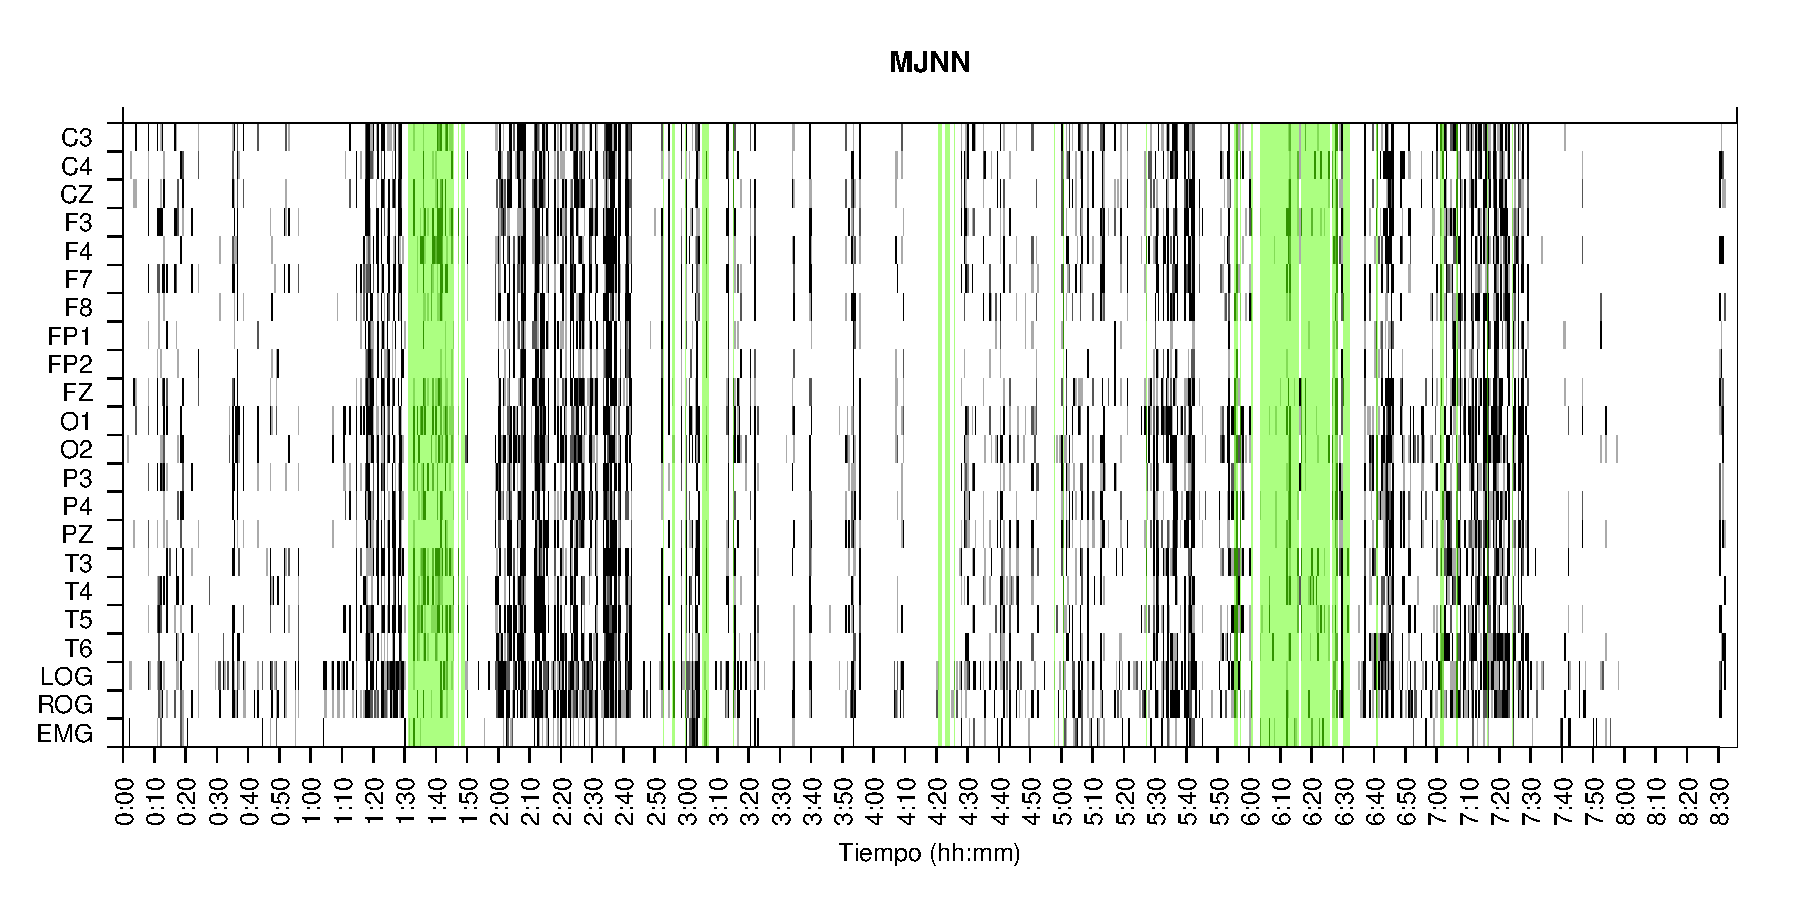
\includegraphics[width=\textwidth]{MJNNVIGILOS_127_mor127_tot1032_esttotal.pdf} 
\caption{Disposici\'on gr\'afica para los resultados del test PSR en el sujeto MJH, 
para 1032 \'epocas de sue\~no y 22 canales. 
En el eje horizontal se muestra el tiempo desde el inicio de registro, en el eje vertical se muestra al 
nombre del canal. 
Se han resaltado con color verde las \'epocas clasificadas como sue\~no MOR (ver texto), que son 127.
Para este gr\'afico se consider\'o con un p-valor cr\'itico de 0.01 para la hip\'otesis
de estacionariedad. Ver texto para m\'as detalles.}
\label{ejemplo1}
\end{figure}

%\begin{figure}
%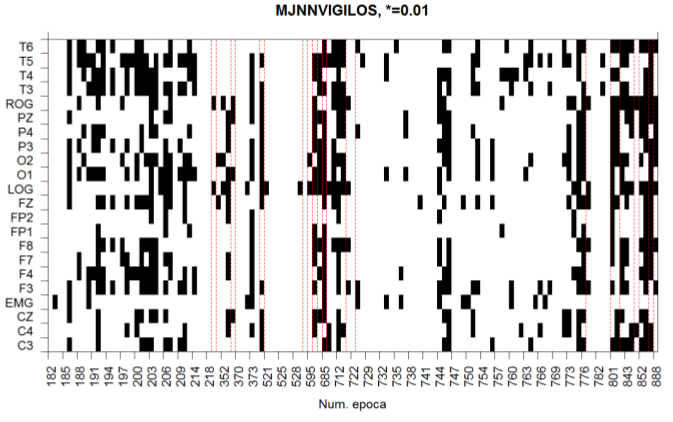
\includegraphics[width=\textwidth]{est02.png} 
%\caption{En este gráfico sólo se ilustran épocas MOR. Las líneas punteadas separan bloques continuos.
%Total de épocas: 1032 , Épocas MOR: 127}
%\label{ejemplo2}
%\end{figure}

%Me siento particularmente orgulloso
%de haber dise\~nado este tipo de gr\'aficos, ya que  organizan datos que ya se ten\'ian
%y dejan la sensaci\'on de portar nueva informaci\'on.

%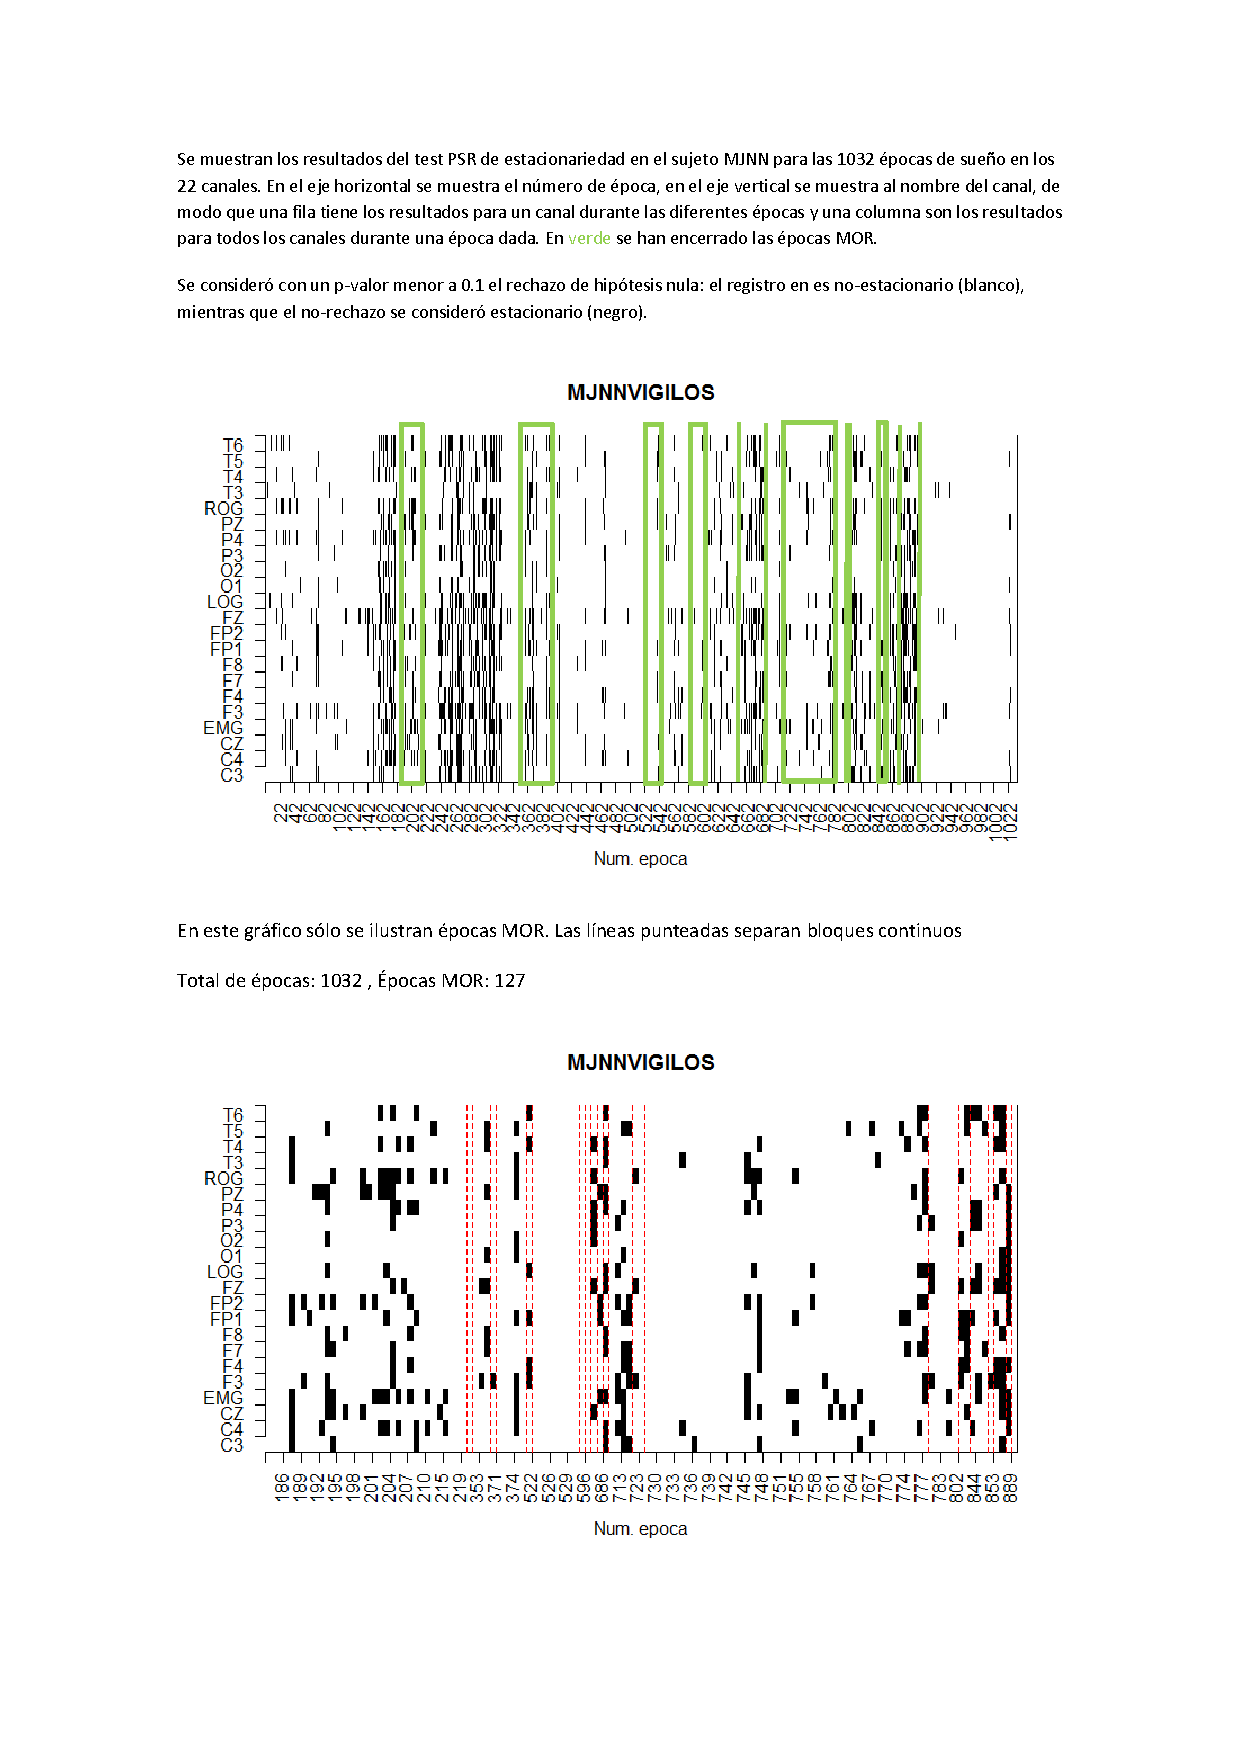
\includepdf[pages={1-},scale=.85]{reporte_de_estacionariedad_170120.pdf}
%
%\afterpage{%
%    \clearpage% Flush earlier floats (otherwise order might not be correct)
%    \thispagestyle{empty}% empty page style (?)
%    \begin{landscape}% Landscape page
%        \centering % Center table
%        \begin{figure}
%            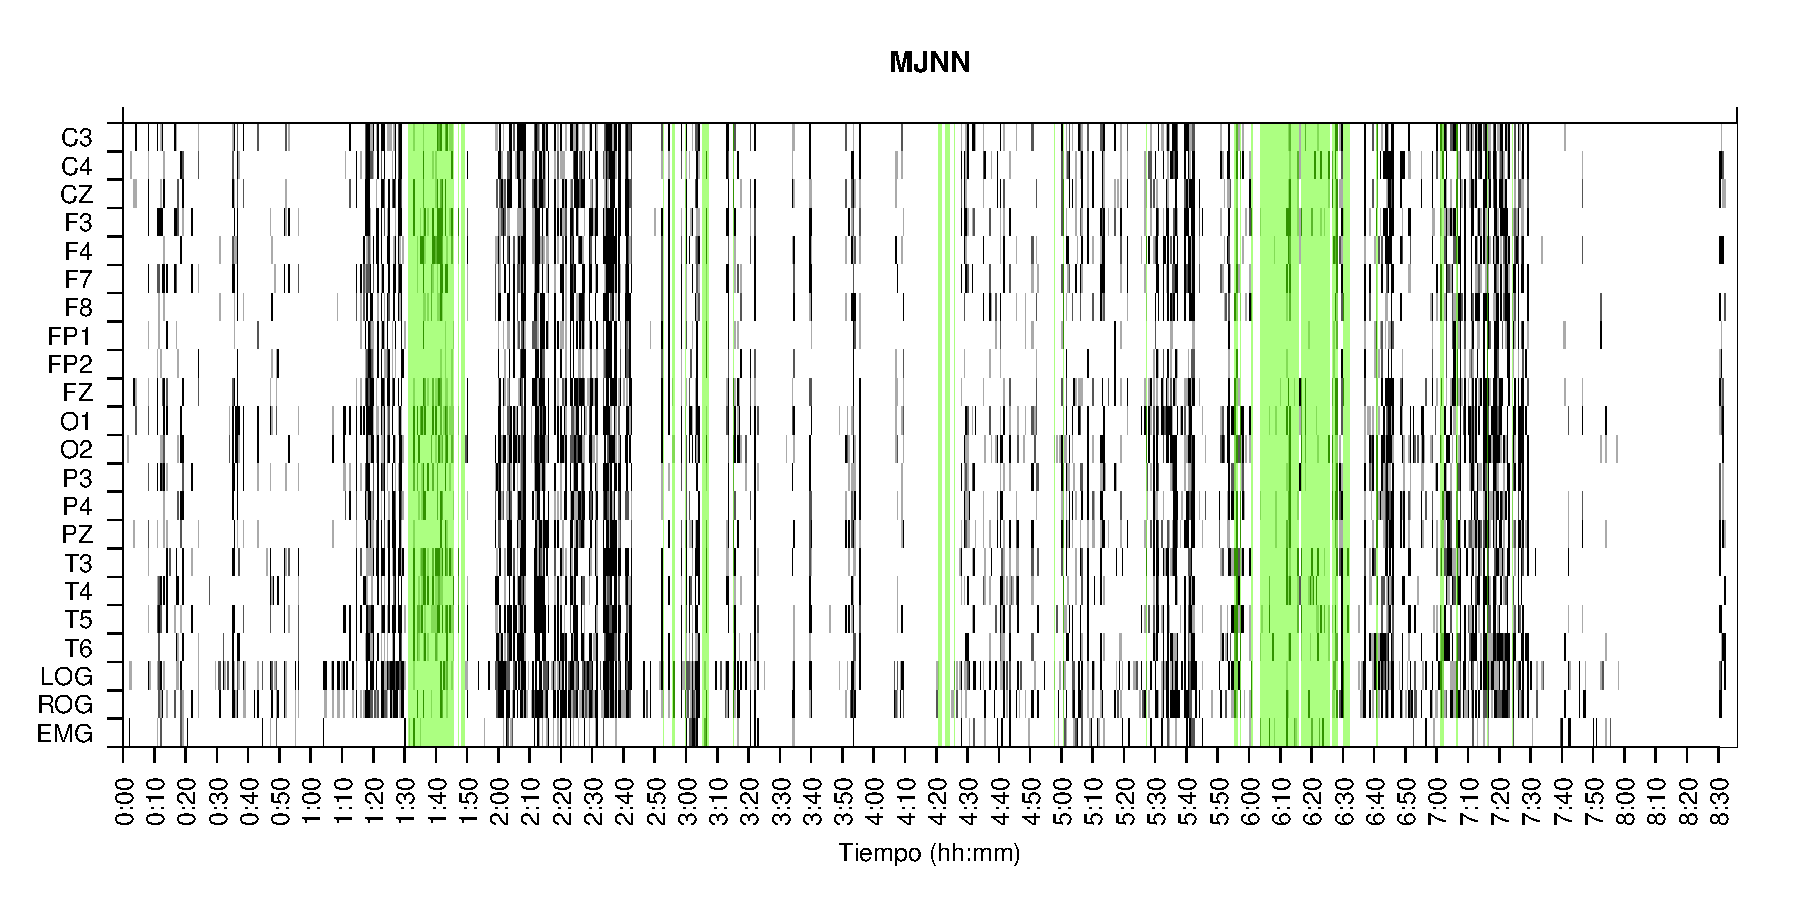
\includegraphics[width=\textwidth]{MJNNVIGILOS_127_mor127_tot1032_esttotal.pdf} 
%            \caption{Total de \'epocas: 1032, \'epocas MOR: 127}
%            %\label{ejemplo1}
%        \end{figure}
%    \end{landscape}
%    \clearpage% Flush page
%}

%%%%%%%%%%%%%%%%%%%%%%%%%%%%%%%%%%%
%%%%%%%%%%%%%%%%%%%%%%%%%%%%%%%%%%%

%\section{Compilados gr\'aficos}
%
%\begin{SidewaysFigure}
%\centering
%\includegraphics[width=\linewidth]
%{./material_bonito170220/MJNNVIGILOS_127_mor127_tot1032_est_total.pdf} 
%\caption{Sujeto: MJNN | Total \'epocas: 1032 | \'Epocas MOR: 127}
%%\label{primera}
%\end{SidewaysFigure}
%\begin{SidewaysFigure}
%\centering
%\includegraphics[width=\linewidth]
%{./material_bonito170220/MJNNVIGILOS_127_mor127_tot127_est_mor.pdf} 
%\caption{Sujeto: MJNN | \'Epocas MOR: 127 | (\'Unicamente \'epocas MOR)}
%%\label{primera}
%\end{SidewaysFigure}
%
%\begin{figure}
%\centering
%\includegraphics[width=\linewidth]
%{./material_bonito170220/porcentaje_bis/MJNNVIGILOS_127_1032_1_bar_porcentaje.pdf} 
%\caption{Sujeto: MJNN | Porcentaje de \'epocas \textit{posiblemente estacionarias}}
%\end{figure}
%
%%%%%%%%%%%%%%%%%%%%%%%%%%%%%%%%%%%%
%%%%%%%%%%%%%%%%%%%%%%%%%%%%%%%%%%%%
%
%\begin{SidewaysFigure}
%\centering
%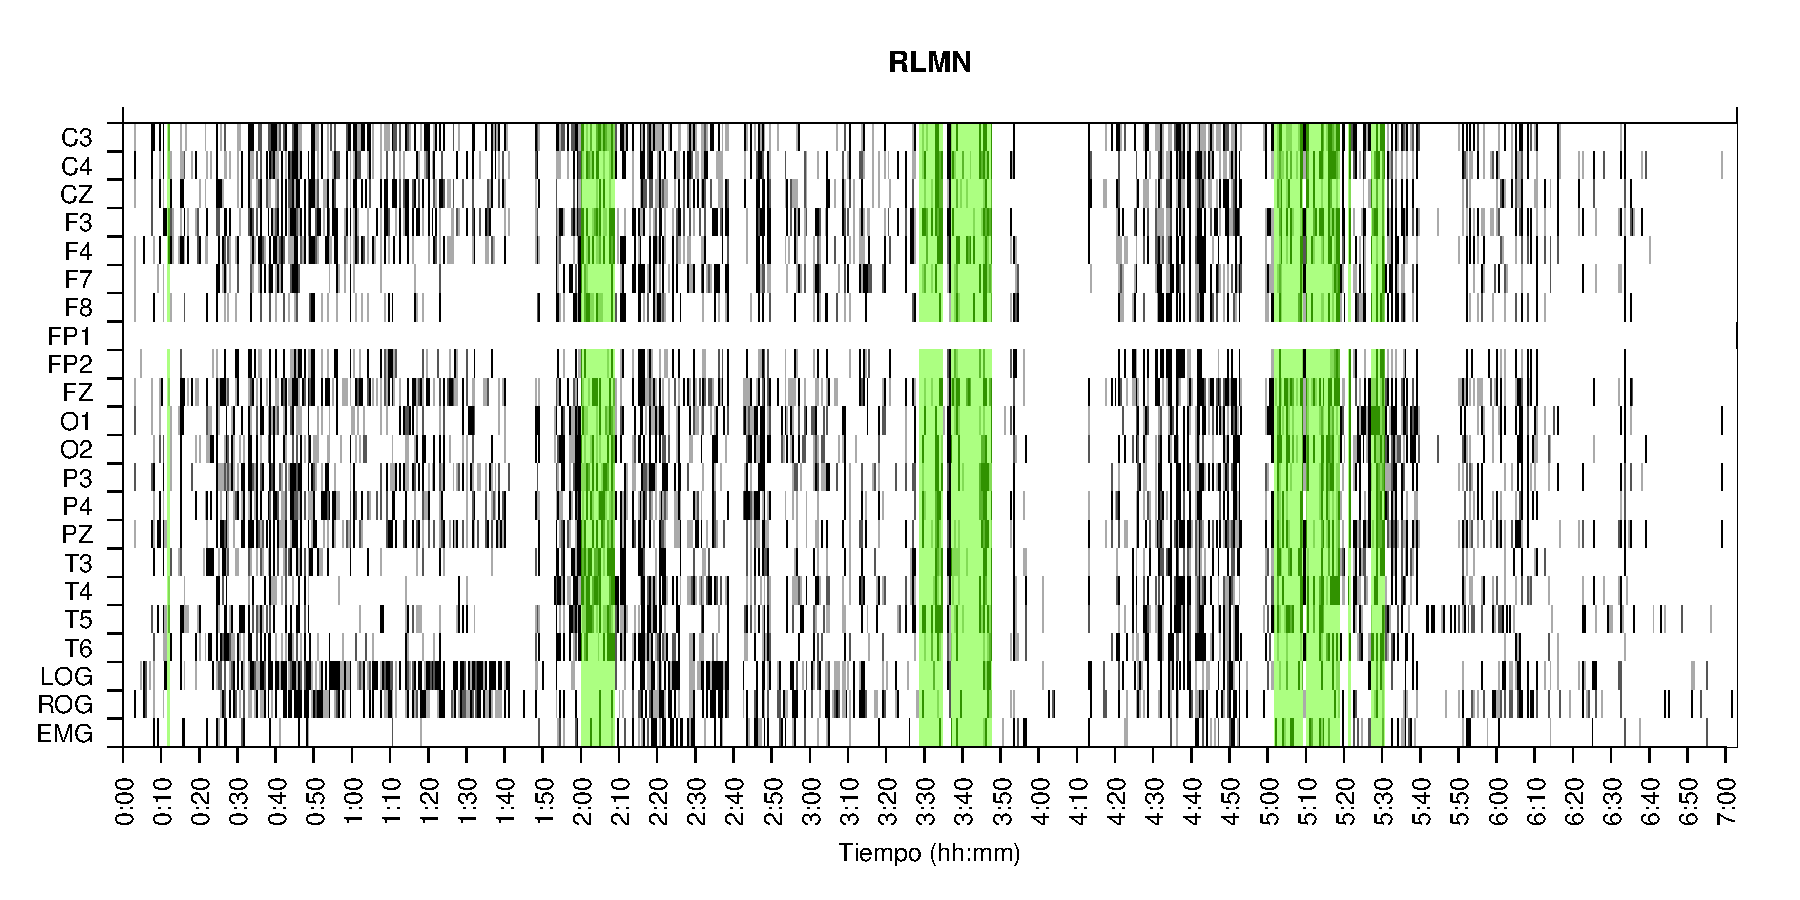
\includegraphics[width=\linewidth]{./material_bonito170220/RLMN10SUE_99_mor99_tot846_est_total.pdf} 
%\caption{Sujeto: RLMN | Total \'epocas: 846 | \'Epocas MOR: 99}
%%\label{primera}
%\end{SidewaysFigure}
%\begin{SidewaysFigure}
%\centering
%\includegraphics[width=\linewidth]
%{./material_bonito170220/RLMN10SUE_99_mor99_tot99_est_mor.pdf} 
%\caption{Sujeto: RLMN | \'Epocas MOR: 99 | (\'Unicamente \'epocas MOR)}
%%\label{primera}
%\end{SidewaysFigure}
%
%\begin{figure}
%\centering
%\includegraphics[width=\linewidth]
%{./material_bonito170220/porcentaje_bis/RLMN10SUE_99_846_1_bar_porcentaje.pdf} 
%\caption{Sujeto: RLMN | Porcentaje de \'epocas \textit{posiblemente estacionarias}}
%\end{figure}
%
%%%%%%%%%%%%%%%%%%%%%%%%%%%%%%%%%%%%
%%%%%%%%%%%%%%%%%%%%%%%%%%%%%%%%%%%%
%
%\begin{SidewaysFigure}
%\centering
%\includegraphics[width=\linewidth]
%{./material_bonito170220/JANASUE_103_mor103_tot907_est_total.pdf} 
%\caption{Sujeto: JANA | Total \'epocas: 907 | \'Epocas MOR: 103}
%%\label{primera}
%\end{SidewaysFigure}
%\begin{SidewaysFigure}
%\centering
%\includegraphics[width=\linewidth]
%{./material_bonito170220/JANASUE_103_mor103_tot103_est_mor.pdf} 
%\caption{Sujeto: JANA | \'Epocas MOR: 103 | (\'Unicamente \'epocas MOR)}
%%\label{primera}
%\end{SidewaysFigure}
%
%\begin{figure}
%\centering
%\includegraphics[width=\linewidth]
%{./material_bonito170220/porcentaje_bis/JANASUE_103_907_1_bar_porcentaje.pdf} 
%\caption{Sujeto: JANA | Porcentaje de \'epocas \textit{posiblemente estacionarias}}
%\end{figure}
%
%%%%%%%%%%%%%%%%%%%%%%%%%%%%%%%%%%%%
%%%%%%%%%%%%%%%%%%%%%%%%%%%%%%%%%%%%
%
%\begin{SidewaysFigure}
%\centering
%\includegraphics[width=\linewidth]
%{./material_bonito170220/CLMN10SUE_132_mor132_tot944_est_total.pdf} 
%\caption{Sujeto: CLMN | Total \'epocas: 944 | \'Epocas MOR: 132}
%%\label{primera}
%\end{SidewaysFigure}
%\begin{SidewaysFigure}
%\centering
%\includegraphics[width=\linewidth]
%{./material_bonito170220/CLMN10SUE_132_mor132_tot132_est_mor.pdf} 
%\caption{Sujeto: CLMN | \'Epocas MOR: 132 | (\'Unicamente \'epocas MOR)}
%%\label{primera}
%\end{SidewaysFigure}
%
%\begin{figure}
%\centering
%\includegraphics[width=\linewidth]
%{./material_bonito170220/porcentaje_bis/CLMN10SUE_132_944_1_bar_porcentaje.pdf} 
%\caption{Sujeto: CLMN | Porcentaje de \'epocas \textit{posiblemente estacionarias}}
%\end{figure}
%
%%%%%%%%%%%%%%%%%%%%%%%%%%%%%%%%%%%%
%%%%%%%%%%%%%%%%%%%%%%%%%%%%%%%%%%%%
%
%\begin{SidewaysFigure}
%\centering
%\includegraphics[width=\linewidth]
%{./material_bonito170220/CLMN10SUE_132_mor132_tot944_est_total.pdf} 
%\caption{Sujeto: JGMN | Total \'epocas: 1207 | \'Epocas MOR: 33}
%%\label{primera}
%\end{SidewaysFigure}
%\begin{SidewaysFigure}
%\centering
%\includegraphics[width=\linewidth]
%{./material_bonito170220/JGMN6SUE_33_mor33_tot33_est_mor.pdf} 
%\caption{Sujeto: CLMN | \'Epocas MOR: 33 | (\'Unicamente \'epocas MOR)}
%%\label{primera}
%\end{SidewaysFigure}
%
%\begin{figure}
%\centering
%\includegraphics[width=\linewidth]
%{./material_bonito170220/porcentaje_bis/JGMN6SUE_33_1207_1_bar_porcentaje.pdf} 
%\caption{Sujeto: JGMN | Porcentaje de \'epocas \textit{posiblemente estacionarias}}
%\end{figure}
%
%%%%%%%%%%%%%%%%%%%%%%%%%%%%%%%%%%%%
%%%%%%%%%%%%%%%%%%%%%%%%%%%%%%%%%%%%
%
%\begin{SidewaysFigure}
%\centering
%\includegraphics[width=\linewidth]
%{./material_bonito170220/RRMNS_114_mor114_tot1244_est_total_bis.pdf} 
%\caption{Sujeto: RRMN | Total \'epocas: 1244 | \'Epocas MOR: 114}
%%\label{primera}
%\end{SidewaysFigure}
%\begin{SidewaysFigure}
%\centering
%\includegraphics[width=\linewidth]
%{./material_bonito170220/RRMNS_114_mor114_tot114_est_mor_bis.pdf} 
%\caption{Sujeto: RRMN | \'Epocas MOR: 114 | (\'Unicamente \'epocas MOR)}
%%\label{primera}
%\end{SidewaysFigure}
%
%\begin{figure}
%\centering
%\includegraphics[width=\linewidth]
%{./material_bonito170220/porcentaje_bis/RRMNS_114_1244_1_bar_porcentaje.pdf} 
%\caption{Sujeto: RRMN | Porcentaje de \'epocas \textit{posiblemente estacionarias}}
%\end{figure}
%
%%%%%%%%%%%%%%%%%%%%%%%%%%%%%%%%%%%%
%%%%%%%%%%%%%%%%%%%%%%%%%%%%%%%%%%%%
%
%\begin{SidewaysFigure}
%\centering
%\includegraphics[width=\linewidth]
%{./material_bonito170220/VCNNS1_200_mor200_tot2584_est_total.pdf} 
%\caption{Sujeto: VCNN | Total \'epocas: 2586 | \'Epocas MOR: 200}
%%\label{primera}
%\end{SidewaysFigure}
%\begin{SidewaysFigure}
%\centering
%\includegraphics[width=\linewidth]
%{./material_bonito170220/VCNNS1_200_mor200_tot200_est_mor.pdf} 
%\caption{Sujeto: VCNN | \'Epocas MOR: 200 | (\'Unicamente \'epocas MOR)}
%%\label{primera}
%\end{SidewaysFigure}
%
%\begin{figure}
%\centering
%\includegraphics[width=\linewidth]
%{./material_bonito170220/porcentaje_bis/VCNNS1_200_2584_1_bar_porcentaje.pdf} 
%\caption{Sujeto: VCNN | Porcentaje de \'epocas \textit{posiblemente estacionarias}}
%\end{figure}
%
%%%%%%%%%%%%%%%%%%%%%%%%%%%%%%%%%%%%
%%%%%%%%%%%%%%%%%%%%%%%%%%%%%%%%%%%%
%
%\begin{SidewaysFigure}
%\centering
%\includegraphics[width=\linewidth]
%{./material_bonito170220/FGHSUE_22_mor22_tot405_est_total.pdf} 
%\caption{Sujeto: FGH | Total \'epocas: 405 | \'Epocas MOR: 22}
%%\label{primera}
%\end{SidewaysFigure}
%\begin{SidewaysFigure}
%\centering
%\includegraphics[width=\linewidth]
%{./material_bonito170220/FGHSUE_22_mor22_tot22_est_mor.pdf} 
%\caption{Sujeto: FGH | \'Epocas MOR: 22 | (\'Unicamente \'epocas MOR)}
%%\label{primera}
%\end{SidewaysFigure}
%
%\begin{figure}
%\centering
%\includegraphics[width=\linewidth]
%{./material_bonito170220/porcentaje_bis/FGHSUE_22_405_1_bar_porcentaje.pdf} 
%\caption{Sujeto: FGH | Porcentaje de \'epocas \textit{posiblemente estacionarias}}
%\end{figure}
%
%%%%%%%%%%%%%%%%%%%%%%%%%%%%%%%%%%%%
%%%%%%%%%%%%%%%%%%%%%%%%%%%%%%%%%%%%
%
%\begin{SidewaysFigure}
%\centering
%\includegraphics[width=\linewidth]
%{./material_bonito170220/GH24031950SUENO_267_mor267_tot3281_est_total.pdf} 
%\caption{Sujeto: GURM | Total \'epocas: 3281 | \'Epocas MOR: 267}
%%\label{primera}
%\end{SidewaysFigure}
%\begin{SidewaysFigure}
%\centering
%\includegraphics[width=\linewidth]
%{./material_bonito170220/GH24031950SUENO_267_mor267_tot267_est_mor.pdf} 
%\caption{Sujeto: GURM | \'Epocas MOR: 267 | (\'Unicamente \'epocas MOR)}
%%\label{primera}
%\end{SidewaysFigure}
%
%\begin{figure}
%\centering
%\includegraphics[width=\linewidth]
%{./material_bonito170220/porcentaje_bis/GH24031950SUENO_267_3281_1_bar_porcentaje.pdf} 
%\caption{Sujeto: GURM | Porcentaje de \'epocas \textit{posiblemente estacionarias}}
%\end{figure}

%%%%%%%%%%%%%%%%%%%%%%%%%%%%%%%%%%%
%%%%%%%%%%%%%%%%%%%%%%%%%%%%%%%%%%%

%%%%%%%%%%%%%%%%%%%%%%%%%%%%%%%%%%%%%%%%%%%%%%%%%%%%%%%%%%%%%%%%%%%%%%%%%%%%%%%%%%%%%%%%%%%%%%%%%%%
%%%%%%%%%%%%%%%%%%%%%%%%%%%%%%%%%%%%%%%%%%%%%%%%%%%%%%%%%%%%%%%%%%%%%%%%%%%%%%%%%%%%%%%%%%%%%%%%%%%